\documentclass{article}
\usepackage[margin=1in]{geometry}
\usepackage{booktabs}
\usepackage{graphicx}
\title{Reporte de carga MQTT}
\author{Autogenerado por mqtt\_stress\_async.py}
\date{}
\begin{document}
\maketitle
\section*{Resumen de la corrida}
\begin{tabular}{ll}\topruleSesión & 20251204-015559-s00000-n00200 \ CSV & ..\textbackslash\{\}20251204-015559-s00000-n00200-metrics.csv \ Dispositivos & 200.000 \ Publicaciones OK & 7.2e+03 \ Publicaciones fallidas & 0.000 \ Latencia promedio (ms) & 6.807 \ Latencia P95 (ms) & 18.626 \ Mensajes por segundo & 30.852 \ Ancho de banda (Mbps) & 0.039 \ Volumen de datos (MB) & 1.081 \ Duración (s) & 233.370 \ \bottomrule\end{tabular}
\subsection*{Gráficos}
\begin{figure}[h]
\centering
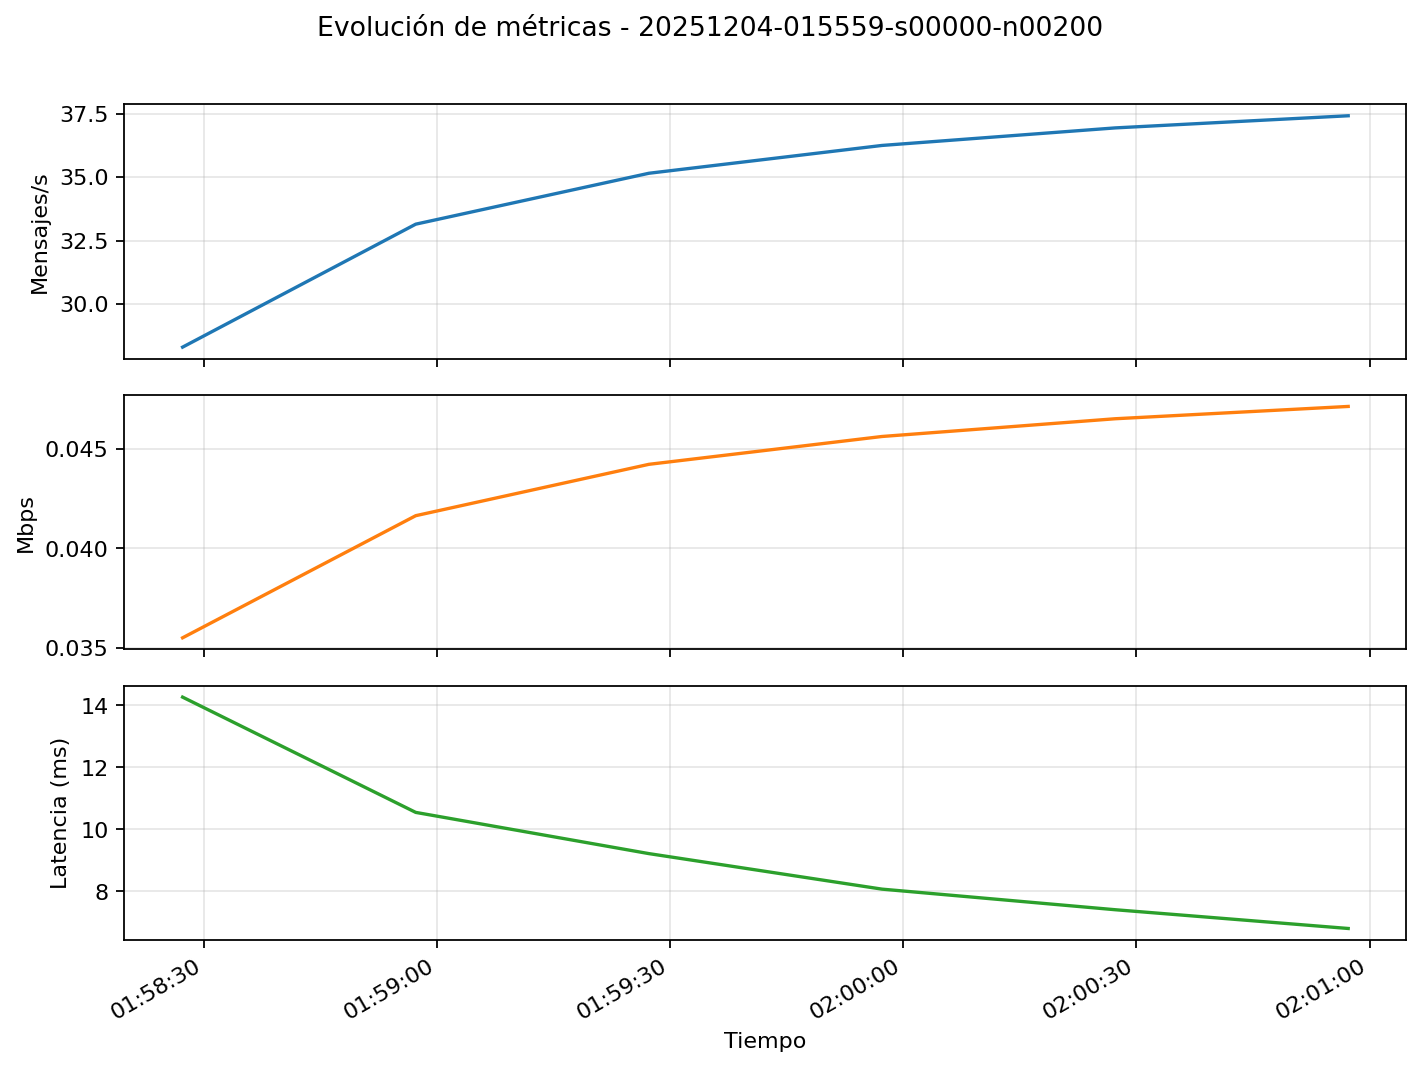
\includegraphics[width=0.9\linewidth]{20251204-015559-s00000-n00200-overview.png}
\caption{Mensajes/s, ancho de banda y latencia promedio.}
\end{figure}

\subsection*{Fuente de datos}
El CSV original se encuentra en \texttt{..\textbackslash\{\}20251204-015559-s00000-n00200-metrics.csv}.\\
Este documento se genera automáticamente tras cada corrida.\
\end{document}
